\subsection{Gamelogic}
La parte di progettazione dei vari componenti di base non è spettata a me, ma ho contribuito, dal secondo sprint in poi, con diverse modifiche e rifattorizzazioni a metodi del model, a volte anche in pair programming con Meshua Galassi (come per il task "Creazione nemici lato model" nel terzo sprint).
Inoltre, contributo significativo all'interno della parte di model sono stati diversi bugfixing nel corso degli sprint.
Le varie classi che ho toccato maggiormente sono: \textit{Arena}, \textit{Enemy}, \textit{MapGenerator}, \textit{MovableEntity}, \textit{Obstacle}, \textit{ObstacleTypes} e \textit{Player}.

Dopo varie rifattorizzazioni susseguite nei vari sprint del mio contributo più significativo rimane:
\begin{itemize}
	\item la rifattorizzazione ai metodi \textit{generateEnemies()}, \textit{generateCollectibles()} e \textit{generateObstacles()} all'interno di \textit{MapGenerator};
	\item la gestione dei record del giocatore ed aggiornamento della classifica in \textit{Player} e \textit{GameState};
	\item la creazione e rifattorizzazione di metodi come \textit{containsCollectible()}, \textit{containsObstacle()}, \textit{containsWall()}, \textit{containsEnemy()} e \textit{containsBullet()} di \textit{Arena};
	\item la creazione di \textit{ObstacleTypes}.
\end{itemize}


\subsection{Gameview}
Durante il primo sprint mi sono occupato della progettazione e realizzazione dei mockup del menù di gioco, andando a creare le principali voci del menù che, ancora nell'ultima versione, sono presenti, quali "\textit{Settings}" e "\textit{Credits}".
Inoltre, per quanto riguarda l'interfaccia di gioco, ho realizzato un prima versione base dell'arena di gioco accessibile attraverso la voce del menù "\textit{Start game}".
Dal quarto sprint ho introdotto anche la voce "\textit{Player rankings}" con relativa scena.
Le varie interfacce dei singoli componenti della view sono stati progettati e realizzati ponendo attenzione a renderli indipendenti dalla piattaforma anche grazie all'utilizzo di file \textit{CSS} e \textit{FXML}.
Quest'ultima tipologia di file è stata prodotta grazie all'utilizzo del tool \textit{Scene Builder}.

Inoltre mi sono occupato della generazione grafica dell'arena, andando a creare le sprite delle varie entità dapprima in modo statico e poi, dal secondo sprint, in modo dinamico a seconda delle informazioni contenute nel model.
In un secondo momento questa generazione grafica è stata rifattorizzata da Giada Gibertoni, andando a snellire la classe \textit{FXGameScene} e portandola alla struttura che ha oggi \ref{view}.

\subsubsection{Scelta della libreria}

Prima della progettazione e implementazione dell'interfaccia mi sono concentrato insieme alla collega Giada Gibertoni sulla ricerca di una libreria grafica da utilizzare.
Il primo risultato di questa ricerca è ricaduto su \textit{ScalaFX} che ricalca lo stile di \textit{JavaFX} però in termini molto più Scala-like.
D'altro canto ci si è accorti quasi subito che è molto scarna di esempi pratici e per questo motivo alla fine abbiamo abbandonato l'idea di utilizzare questa libreria.
La ricerca è proseguita su altre librerie tutte scartate o per il medesimo motivo o perché non davano la possibilità di definire l'interfaccia grafica tramite file esterni, limitando il tutto a dover disegnare la GUI tramite classi.
Alla fine si è optato per JavaFX, soprattutto perché offre tanti esempi reperibili online grazie ad una community molto attiva e anche perché offre un'integrazione con file esterni come FXML.

\subsubsection{Finestra generica e implementazione in JavaFX}

Data questa incertezza iniziale sulla scelta della libreria grafica, sono andato a creare una finestra generica grazie alla quale un eventuale futuro cambio di libreria non avrebbe portato comportamenti inattesi nel comportamento di base della finestra.
Una volta definite le funzionalità di base nell'interfaccia \textit{Window}, questa sarà implementata da \textit{FXWindow} che va a creare una finestra conforme agli standard di JavaFX.

\begin{figure}[H]
  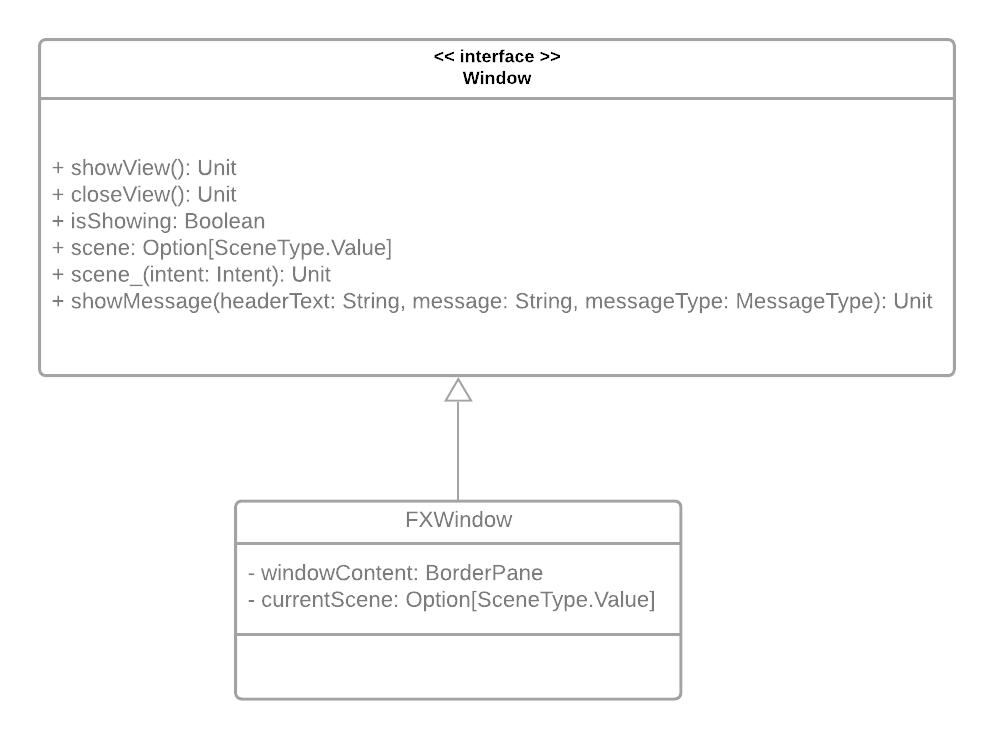
\includegraphics[width=15cm]{../res/6-implementazione/chiana/UML_Window.png}
  \caption{Interfaccia Window e FXWindow che la implementa.}
  \label{windowClass}
\end{figure}

\subsubsection{Navigazione e scene}
La navigazione tra le schermate viene permesso grazie al metodo \textit{scene\textunderscore()} che va a creare la nuova scena e a notificare all'observer (\textit{GameManager}) che deve cambiare la scena con la nuova.
La decisione su che scena creare viene presa sul tipo di scena (\textit{SceneType}), un'\textit{Enumeration} passata come parametro all'\textit{Intent} (classe che rappresenta l'intento di cambiare la scena corrente con un'altra).

\subsubsection{Arena di gioco}
Mi sono inoltre occupato della creazione dell'interfaccia di gioco, andando a creare visualmente l'arena che il giocatore vedrà mentre gioca, all'interno di \textit{FXGameScene}.
Qui ogni punto dell'arena logica viene tradotto in una piastrella alla quale viene assegnata una certa sprite a seconda della tipologia dell'entità che è presente su tale punto (metodo \textit{createArena()}).
Queste piastrelle vengono regolarmente aggiornate ed allineate con la parte logica del programma tramite il metodo \textit{nextStep()} di \textit{GameLoop}.
La realizzazione di FXGameScene è stata incrementale durante tutto lo sviluppo del gioco, tant'è che ha subito diverse modifiche e aggiunte da diversi componenti del gruppo.

\subsection{Gamemanager}
La parte di gamemanager, come per la parte di gamelogic, la sono andato a toccare diverse volte, ma solo con piccole modifiche e rifattorizzazioni.
I contributi più significativi che ho dato in questa parte del progetto si possono suddividere in: \textit{PreferencesHandler} e \textit{caricamento e salvataggio della classifica di gioco}.

\subsubsection{PreferencesHandler}
Viene utilizzata per salvare le preferenze dell'utente come il nome e la difficoltà di gioco attraverso l'uso di \textit{Java Preferences API}.
Il salvataggio e la serializzazione di queste impostazioni vengono fatte attraverso l'estensione \textit{lift-json-ext} che verrà poi utilizzata anche per salvare la classifica di gioco.

\subsubsection{Classifica di gioco}
La classifica di gioco viene salvata in un file JSON tramite la \textit{PrintWriter} di \textit{java.io} con la seguente struttura: \ref{json}

\begin{figure}[H]
  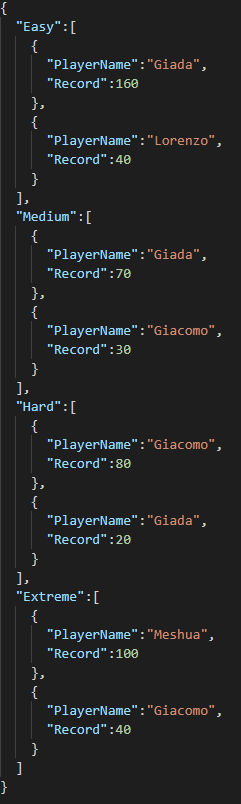
\includegraphics[width=5cm]{../res/6-implementazione/chiana/json.png}
  \caption{Struttura del file rank.json}
  \label{json}
\end{figure}

Questo file viene letto tramite il metodo \textit{loadPlayerRankings()} di \textit{GameManager} andando a creare una mappa che come chiave presenta il nome della difficoltà e come valore un'altra mappa che, a sua volta, come chiave ha il nome del giocatore e come valore il suo record.

<<qualcosa per farlo capire>>

Questa mappa viene salvata in \textit{GameState} (all'interno di gamelogic) e aggiornata dinamicamente durante il gioco.

Alla fine di ogni partita la mappa viene salvata nel file JSON attraverso il metodo \textit{savePlayerRankings()}.

\subsection{Utilities}
Nei vari sprint a seconda dell'esigenza sono andato a creare:
\begin{itemize}
	\item Animations: utilizzata per creare un animazione di fade-in o fade-out tra le varie scene;
	\item Intent: classe che rappresenta l'intento di cambiare la scena corrente con un'altra;
	\item MessageTypes: un sailed trait che rappresenta i vari tipi di messaggi di una finestra di dialogo;
	\item ViewLoader: permette il caricamento, e quindi l'utilizzo, di layout in formato \textit{.fxml};
	\item WindowSize: contiene le dimensioni della finestra del menù principale e di quella di gioco.
		
\end{itemize}

\subsection{Test}
Per quanto riguarda la parte di testing mi sono occupato di andare a testare le classi \textit{Player}, \textit{Hero}, \textit{Enemy} e \textit{Bullet} con \textit{AnyFlatSpec} come tipologia di sintassi.

Per ogni entità sono andato a testare le caratteristiche principali come ad esempio la direzione del movimento, le collisioni, eventuali decrementi o incrementi di vita o di punteggio e così via.
L'unico inconveniente di questo approccio era dato dalla casualità di creazione dell'arena di gioco che poteva far fallire alcuni test come, ad esempio, testare il movimento in una certa direzione.
In questo caso si poteva presentare il caso in cui, nel punto in cui si doveva muovere l'entità, era presente un'altra entità finendo per colliderci e risultando di consenguenza non essersi mossa.
Per ovviare a questo problema ho optato nella creazione di una classe builder \textit{StaticArena} nella quale l'arena generata casualmente viene svuotata e impostata con delle entità in determinati punti passatagli come parametri, permettendo così di creare una scena ad hoc per il test da eseguire.

\subsection{Environment}
Dell'ambiente di sviluppo mi sono occupato di impostare in sbt i plugin \textit{ScalaStyle}, per il controllo dello stile, e \textit{sbt-assembly}, per il deploy del file jar.
Inoltre mi sono occupato della configurazione di Travis CI, andando ad impostare la versione di Scala, la directory del progetto, e la versione della JDK da utilizzare.
